\documentclass[12pt,a4paper]{article}
\usepackage[utf8]{inputenc}
\usepackage[T1]{fontenc}
\usepackage{lmodern}
\usepackage{amsmath,amssymb}
\usepackage{tikz}
\usepackage{geometry}
\geometry{margin=2.5cm}

\begin{document}

\begin{center}
\Large \textbf{Zajęcia 2: wielokąt rozwiązań cząstkowych i jego „środki”}
\end{center}

\section*{Układ i trójkąt rozwiązań cząstkowych}

Rozważamy sprzeczny układ równań:
\[
\begin{cases}
(1)\; 2x + y = 5,\\
(2)\; x - y = 1,\\
(3)\; x + y = 2.
\end{cases}
\]
Każda para równań daje jednoznaczne rozwiązanie:
\[
\begin{aligned}
&(1)\wedge(2): && A=(2,1),\\
&(1)\wedge(3): && B=(3,-1),\\
&(2)\wedge(3): && C=\left(\tfrac{3}{2},\tfrac{1}{2}\right).
\end{aligned}
\]
Wielościan wypukły (tutaj trójkąt) to
\[
\Delta=\mathrm{conv}\{A,B,C\}.
\]

\paragraph{Opis nierównościami (prosto z równań).}
Wnętrze trójkąta wyznaczają trzy półprzestrzenie:
\[
\boxed{\;2x+y\le 5,\quad x-y\ge 1,\quad x+y\ge 2\;}
\]
(granice to odpowiednio proste (1), (2), (3)).

\section*{Rysunek}

\begin{center}
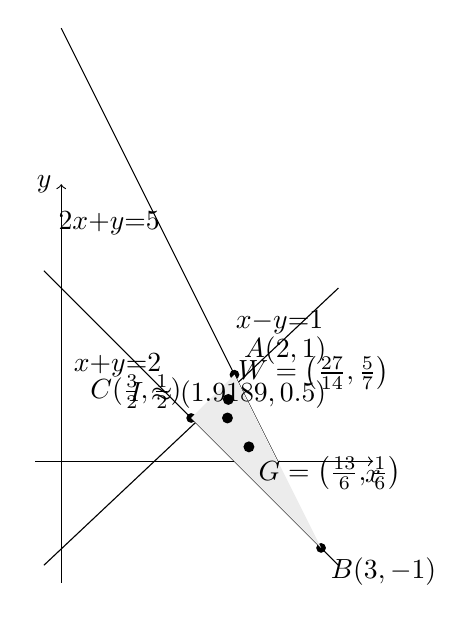
\begin{tikzpicture}[scale=1.1]
  % osie
  \draw[->] (-0.3,0) -- (3.6,0) node[below] {$x$};
  \draw[->] (0,-1.4) -- (0,3.2) node[left] {$y$};

  % proste
  % (1) 2x + y = 5 -> y = 5 - 2x
  \draw (-0.0,5) -- (2.5,0) node[pos=0.5, above left] {$2x{+}y{=}5$};
  % (2) x - y = 1 -> y = x - 1
  \draw (-0.2,-1.2) -- (3.2,2) node[pos=0.8, above] {$x{-}y{=}1$};
  % (3) x + y = 2 -> y = 2 - x
  \draw (-0.2,2.2) -- (3.2,-1.2) node[pos=0.25, below] {$x{+}y{=}2$};

  % wierzchołki
  \fill (2,1) circle (1.6pt) node[above right] {$A(2,1)$};
  \fill (3,-1) circle (1.6pt) node[below right] {$B(3,-1)$};
  \fill (1.5,0.5) circle (1.6pt) node[above left] {$C(\tfrac{3}{2},\tfrac{1}{2})$};

  % trójkąt
  \fill[gray!15] (2,1) -- (3,-1) -- (1.5,0.5) -- cycle;

  % centroid G
  \coordinate (G) at ({(2+3+1.5)/3},{(1-1+0.5)/3});
  \fill (G) circle (1.8pt) node[below right] {$G=\bigl(\tfrac{13}{6},\tfrac{1}{6}\bigr)$};

  % weighted center W (det^2)
  \coordinate (W) at ({27/14},{5/7});
  \fill (W) circle (1.8pt) node[above right] {$W=\bigl(\tfrac{27}{14},\tfrac{5}{7}\bigr)$};

  % incenter I (Chebyshev center) ~ (1.9189, 0.5)
  \coordinate (I) at (1.9189,0.5);
  \fill (I) circle (1.8pt) node[above] {$I\approx(1.9189,0.5)$};

\end{tikzpicture}
\end{center}

\section*{„Środki” i obliczenia}

\subsection*{(a) Centroid (środek mas wierzchołków)}
\[
G=\frac{A+B+C}{3}
=\left(\frac{2+3+\tfrac{3}{2}}{3},\,\frac{1+(-1)+\tfrac{1}{2}}{3}\right)
=\left(\frac{13}{6},\,\frac{1}{6}\right).
\]

\subsection*{(b) Ważony środek (przykład: wagi z \(\det^2\))}
Niech wagi pochodzą z podukładów: \(w_{12}\propto \det(A_{12})^2,\; w_{13}\propto \det(A_{13})^2,\; w_{23}\propto \det(A_{23})^2\).
Dla macierzy
\(
A=\begin{bmatrix}2&1\\[2pt]1&-1\\[2pt]1&1\end{bmatrix}
\)
i par wierszy dostajemy
\[
|\det A_{12}|=3,\quad |\det A_{13}|=1,\quad |\det A_{23}|=2
\Rightarrow (w_{12},w_{13},w_{23})\propto (9,1,4).
\]
Wtedy
\[
W=\frac{9A+1B+4C}{9+1+4}
=\left(\frac{27}{14},\,\frac{5}{7}\right)\approx(1.9286,0.7143).
\]
\emph{Uwaga.} Ten wybór wag daje tu punkt będący klasycznym rozwiązaniem w sensie najmniejszych kwadratów.

\subsection*{(c) Punkt o najmniejszej energii (najmniejszej normie Euklidesowej) w \(\Delta\)}
Szukamy \(\displaystyle \arg\min_{x\in\Delta}\|x\|_2\).
Rzut prostopadły z \(0\) na proste krawędzi daje odpowiednio:
\[
\begin{aligned}
&\text{na } 2x+y=5:\; (2,1)=A\ \text{(leży na odcinku)},\\
&\text{na } x-y=1:\; (1/2,-1/2)\ \text{(poza odcinkiem \(AC\))},\\
&\text{na } x+y=2:\; (1,1)\ \text{(poza odcinkiem \(BC\))}.
\end{aligned}
\]
Zatem kandydatami są wierzchołki; porównując normy
\[
\|A\|=\sqrt{5},\quad \|B\|=\sqrt{10},\quad \|C\|=\sqrt{2.5}
\]
minimalna jest w \(C\). Stąd
\[
\boxed{\;x_{\min\|\,\cdot\,\|} = C=\left(\tfrac{3}{2},\tfrac{1}{2}\right)\;}
\]

\subsection*{(d) Środek Czebyszewa (incenter)}
Dla trójkąta jest to środek okręgu wpisanego. Jeśli \(a=|BC|=\sqrt{4.5}=3/\sqrt{2}\), \(b=|AC|=\sqrt{0.5}=1/\sqrt{2}\), \(c=|AB|=\sqrt{5}\),
to
\[
I=\frac{aA+bB+cC}{a+b+c},\qquad
r=\frac{2\Delta}{a+b+c},
\]
gdzie \(\Delta\) to pole trójkąta. Stąd
\[
I=\left(\frac{\tfrac{3}{2}\,(3\sqrt{2}+\sqrt{5})}{\,2\sqrt{2}+\sqrt{5}\,},\;\frac{1}{2}\right)\approx(1.9189,\,0.5),
\quad
\Delta=\tfrac{3}{4},\quad
r=\frac{3/2}{\,2\sqrt{2}+\sqrt{5}\,}\approx 0.2963.
\]

\subsection*{(e) Środek analityczny (analytic center)}
Dla opisu \(\{\,2x{+}y\le 5,\; -x{+}y\le -1,\; -x{-}y\le -2\,\}\) środek analityczny minimalizuje
\[
\phi(x,y)=-\log(5-2x-y)-\log(x-y-1)-\log(x+y-2).
\]
Warunek stacjonarności daje
\(\;\frac{(2,1)}{5-2x-y}+\frac{(-1,1)}{x-y-1}+\frac{(-1,-1)}{x+y-2}=0\).
Rozwiązanie spełnia
\[
5-2x-y=\tfrac{1}{2},\quad x-y-1=1,\quad x+y-2=\tfrac{1}{3}
\]
i w efekcie
\[
\boxed{\;x_{\mathrm{an}}=\left(\tfrac{13}{6},\tfrac{1}{6}\right)\;}
\]
(tutaj zbiega się to z centroidem, co \emph{nie jest regułą} – środek analityczny zależy od skalowania nierówności).

\bigskip
\noindent
\textbf{Podsumowanie.} Dla trójkąta \(ABC\) z powyższego przykładu:
\[
\begin{aligned}
&G=\left(\tfrac{13}{6},\tfrac{1}{6}\right),\qquad
W=\left(\tfrac{27}{14},\tfrac{5}{7}\right),\qquad
x_{\min\|\,\cdot\,\|}=C=\left(\tfrac{3}{2},\tfrac{1}{2}\right),\\[4pt]
&I=\left(\frac{\tfrac{3}{2}(3\sqrt{2}+\sqrt{5})}{2\sqrt{2}+\sqrt{5}},\;\tfrac12\right),\qquad
x_{\mathrm{an}}=\left(\tfrac{13}{6},\tfrac{1}{6}\right).
\end{aligned}
\]

\end{document}
